% ---------------------------------------------------------------------
% Cloned from the HES-SO//Master canvas 2019
% ---------------------------------------------------------------------


\chapter{Experiments \& Results}
\label{chap:experiments-results}
With the goal of getting a hold on the Word2Vec technology and as a complement to the analysis chapter \ref{chap:analysis}, the following are the experiments made during the deepening project and theirs results.

\section{Environments}
The language used during the whole chapter is Python with the Gensim framework.

\subsection{Jupyter Notebook}


\subsection{Local Machine}
\subsection{Amazon Web Services}
\subsection{iColab-gpu2}
\subsection{CPU Dedicated Machine}


\section{Gensim Framework}


\subsection{Memory Issues}
Memory allocation with multi-core. The problem is occurring during the merge of the cores. Indeed, my current machine has 128GB ram, and the dataset weights about 16GB in the memory, and each core during merging is processing at least the same amount, plus the processed informations.\\ 

\begin{figure}[htbp]
\centering
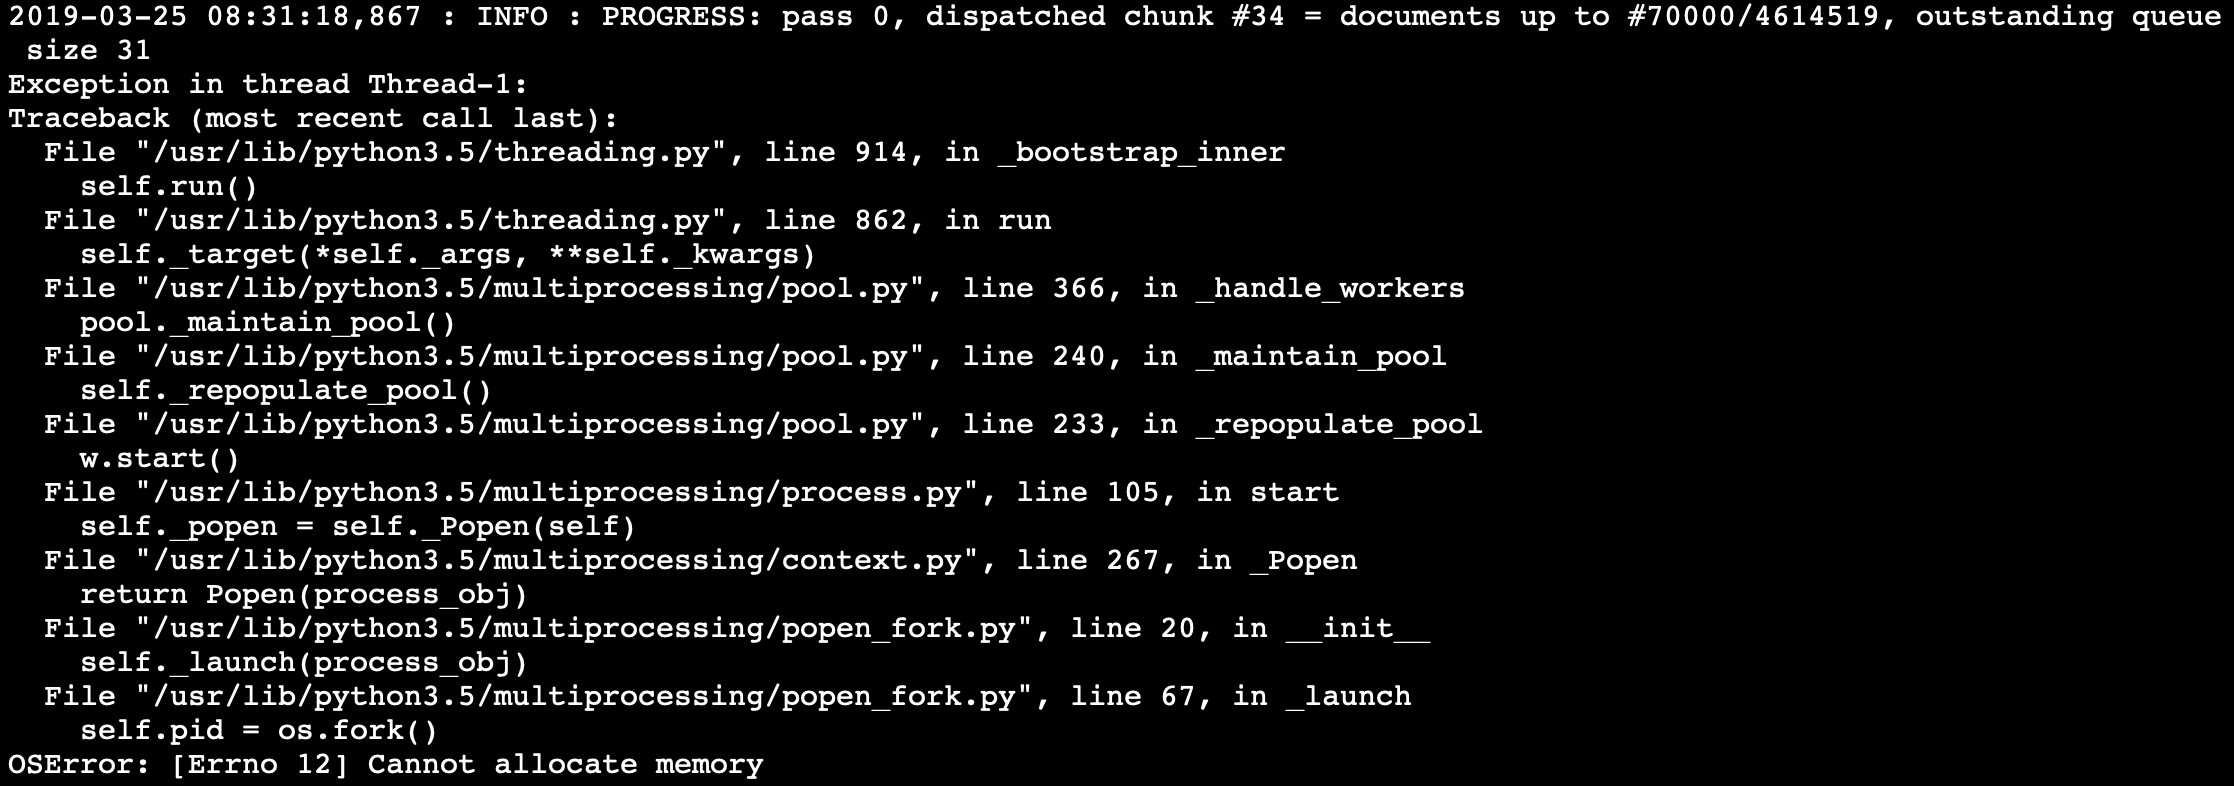
\includegraphics[width=\linewidth]{99-imgs/gensim_memory_allocation_error}
\caption{Error 1}
\label{fig:error-1}
\end{figure}

\begin{figure}[htbp]
\centering
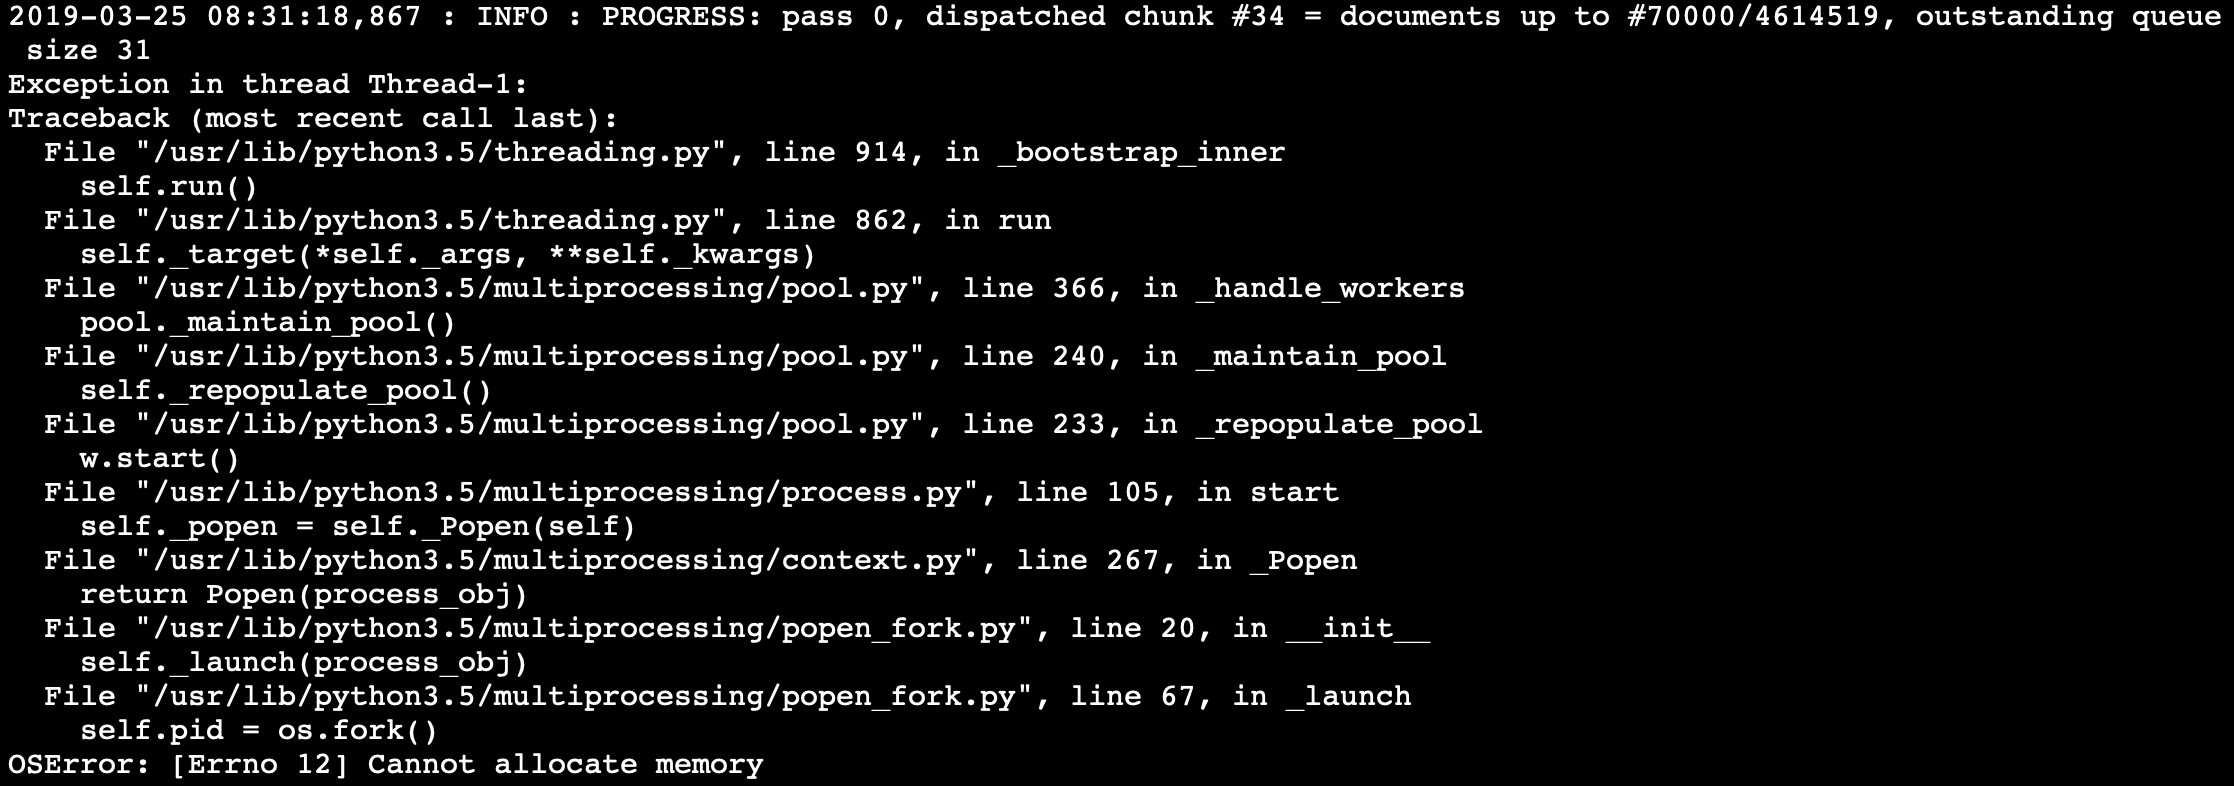
\includegraphics[width=\linewidth]{99-imgs/gensim_memory_allocation_error}
\caption{Error 2}
\label{fig:error-2}
\end{figure}

\section{Materials}

\section{Products}

\section{Word2Vec}
\subsection{Proverbs}
\subsection{Visual Representation}
\subsection{Benchmarks}
\subsection{CPUs vs RAM}

\section{Doc Embedding: Seq2Seq}
\section{Chatbot}
\section{Proactivity}



